\begin{figure}
\centering
\vspace{-1mm}
	\begin{subfigure}[b]{0.65 \textwidth}
	\begin{scriptsize}
	1. Consider a replica containing $\{\eta_1,\eta_2,\eta_3\}$ when an
	operation $op$ arrives with a \textsf{UB} contract according to
	which, any operation
	witnessing $\eta_1$, must also witness $\eta_4$.
	\\2. A violation of the contract occurs if $op$
	witnesses $\eta_1$ (left), whereas a 
	filteration mechanism enforces the contract
	(right).
	\end{scriptsize}
	\end{subfigure}
	~
	\begin{subfigure}[b]{0.298 \textwidth}
	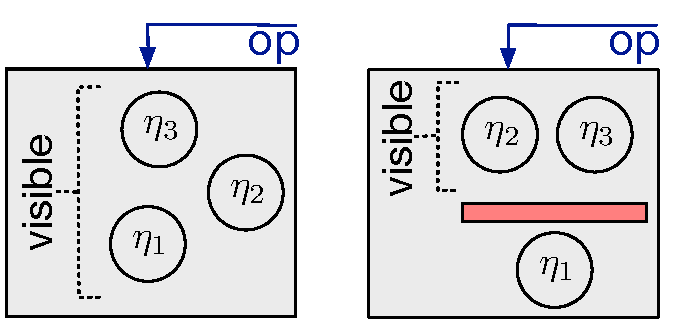
\includegraphics[scale=0.36]{Figures/ub.pdf}
	\end{subfigure}
	\caption{Filteration and \UB{} contracts}
\vspace{-5mm}
\label{fig:ub}
\end{figure}
